\mchapter{ارزیابی و معیارهای سنجش عملکرد}

ارزیابی مدل‌ها یکی از مراحل حیاتی در فرآیند یادگیری عمیق است چرا که تنها از طریق ارزیابی می‌توان عملکرد مدل را سنجید، نقاط قوت و ضعف آن را شناسایی کرد و در نهایت تصمیمات لازم برای بهبود مدل را اتخاذ نمود.

در این فصل، ابتدا به معرفی معیارهای مختلف برای ارزیابی مدل‌های دسته‌بندی چندبرچسبی می‌پردازیم. این معیارها به ما کمک می‌کنند تا از زوایای مختلفی عملکرد مدل را بسنجیم و درک عمیق‌تری از نحوه عملکرد مدل در مسائلی با چندین برچسب همزمان پیدا کنیم. سپس، با یک مثال عملی نحوه استفاده از این معیارها برای ارزیابی مدل را توضیح خواهیم داد. این مثال به شما کمک خواهد کرد تا بهتر بتوانید این معیارها را در مسائل واقعی پیاده‌سازی کنید و به طور مؤثرتری مدل خود را مورد ارزیابی قرار دهید.

معیارهایی که در این فصل معرفی می‌شوند، هر کدام به نوع خاصی از عملکرد مدل توجه دارند و می‌توانند در شرایط مختلفی مفید واقع شوند. برای مثال، برخی از این معیارها بر توانایی مدل در تشخیص تمام برچسب‌های مرتبط تمرکز دارند، در حالی که برخی دیگر به دقت پیش‌بینی‌های مدل اهمیت می‌دهند. با استفاده از این معیارها، می‌توان مدلی را که بهترین تعادل را بین دقت و بازخوانی برقرار می‌کند، شناسایی کرد.

در ادامه این فصل، با جزئیات بیشتری با این معیارها آشنا می‌شویم و یاد می‌گیریم که چگونه از آنها برای ارزیابی مدل‌های دسته‌بندی چندبرچسبی استفاده کنیم. این دانش به شما کمک خواهد کرد تا به عنوان یک محقق یا مهندس یادگیری عمیق، بتوانید مدل‌های کارآمدتر و مؤثرتری بسازید.
\section{معیارهای ارزیابی}

در دسته‌بندی چندبرچسبی\LTRfootnote{Multi-Label classification}، معیارهای ارزیابی مختلفی برای سنجش عملکرد مدل وجود دارد. در ادامه به برخی از این معیارها اشاره شده است.
\\
در معیار های زیر $N$ تعداد نمونه‌ها، $Y_i$ مجموعه برچسب‌های واقعی و $\hat{Y}_i$ مجموعه برچسب‌های پیش‌بینی‌شده برای نمونه $i$ است:


\subsection{دقت \protect\LTRfootnote{Accuracy}}

دقت در دسته‌بندی چندبرچسبی به صورت زیر تعریف می‌شود:
\cite{evaluationMetric}
\begin{equation}
	\text{دقت} = \frac{1}{N} \sum_{i=1}^{N} \frac{|Y_i \cap \hat{Y}_i|}{|Y_i \cup \hat{Y}_i|}
	\label{eq:accuracy}
\end{equation}
\subsection{دقت نمونه \protect\LTRfootnote{Example-Based Precision}}

دقت نمونه نشان می‌دهد که از میان برچسب‌های پیش‌بینی شده، چه نسبتی از آنها واقعاً صحیح بوده‌اند. این معیار برای ارزیابی دقت پیش‌بینی‌های مدل مفید است.
\cite{evaluationMetric}

\begin{equation}
	\text{دقت نمونه} = \frac{1}{N} \sum_{i=1}^{N} \frac{|Y_i \cap \hat{Y}_i|}{|\hat{Y}_i|}
	\label{eq:precision}
\end{equation}
\subsection{بازخوانی نمونه \protect\LTRfootnote{Example-Based Recall}}

بازخوانی نمونه نشان می‌دهد که از میان برچسب‌های واقعی، چه نسبتی از آنها توسط مدل پیش‌بینی شده‌اند. این معیار برای ارزیابی توانایی مدل در شناسایی تمام برچسب‌های مرتبط مهم است.
\cite{evaluationMetric}

\begin{equation}
	\text{بازخوانی نمونه} = \frac{1}{N} \sum_{i=1}^{N} \frac{|Y_i \cap \hat{Y}_i|}{|Y_i|}
	\label{eq:recall}
\end{equation}
\subsection{امتیاز \lr{F1} نمونه \protect\LTRfootnote{Example-Based F1 Score}}

امتیاز \lr{F1} نمونه میانگین هارمونیک دقت و بازخوانی نمونه است. این معیار تعادلی بین دقت و بازخوانی ایجاد می‌کند و برای ارزیابی کلی عملکرد مدل مفید است.
\cite{evaluationMetric}

\begin{equation}
	\text{امتیاز \lr{F1} نمونه} = \frac{1}{N} \sum_{i=1}^{N} \frac{2 \times |Y_i \cap \hat{Y}_i|}{|Y_i| + |\hat{Y}_i|}
	\label{eq:f1}
\end{equation}
\subsection{دقت خرد \protect\LTRfootnote{Micro-Averaged Precision}}

دقت خرد، دقت کلی مدل را در تمام نمونه‌ها و برچسب‌ها محاسبه می‌کند. این معیار برای ارزیابی عملکرد کلی مدل در تمام کلاس‌ها مفید است.
\cite{evaluationMetric}

\begin{equation}
	\text{دقت خرد} = \frac{\sum_{i=1}^{N} |Y_i \cap \hat{Y}_i|}{\sum_{i=1}^{N} |\hat{Y}_i|}
	\label{eq:ma-precision}
\end{equation}
\subsection{بازخوانی خرد \protect\LTRfootnote{Micro-Averaged Recall}}

بازخوانی خرد، بازخوانی کلی مدل را در تمام نمونه‌ها و برچسب‌ها محاسبه می‌کند. این معیار نشان می‌دهد که مدل تا چه حد توانسته است تمام برچسب‌های مرتبط را در کل مجموعه داده شناسایی کند.
\cite{evaluationMetric}

\begin{equation}
	\text{بازخوانی خرد} = \frac{\sum_{i=1}^{N} |Y_i \cap \hat{Y}_i|}{\sum_{i=1}^{N} |Y_i|}
	\label{eq:ma-recall}
\end{equation}
\subsection{امتیاز \lr{F1} خرد \protect\LTRfootnote{Micro-Averaged F1 Score}}

امتیاز \lr{F1} خرد، میانگین هارمونیک دقت خرد و بازخوانی خرد است. این معیار یک ارزیابی متعادل از عملکرد کلی مدل در تمام کلاس‌ها ارائه می‌دهد و برای مقایسه مدل‌های مختلف مفید است.
\cite{evaluationMetric}

\begin{equation}
	\text{امتیاز \lr{F1} خرد} = \frac{2 \times \text{دقت خرد} \times \text{بازخوانی خرد}}{\text{دقت خرد} + \text{بازخوانی خرد}}
	\label{eq:ma-f1}
\end{equation}
این معیارها برای سنجش عملکرد مدل در دسته‌بندی چندبرچسبی و شناسایی نقاط قوت و ضعف آن موثر اند.

\section{نحوه ارزیابی مدل}

برای ساده تر کردن موضوع یه مسئله چهار کلاسه را در نظر بگیرید، خروجی مدل به صورت یک آرایه چهار تایی می‌باشد.به شکل \ref{fig:evaluate} توجه کنید:
\begin{figure}[H]
	\centering
	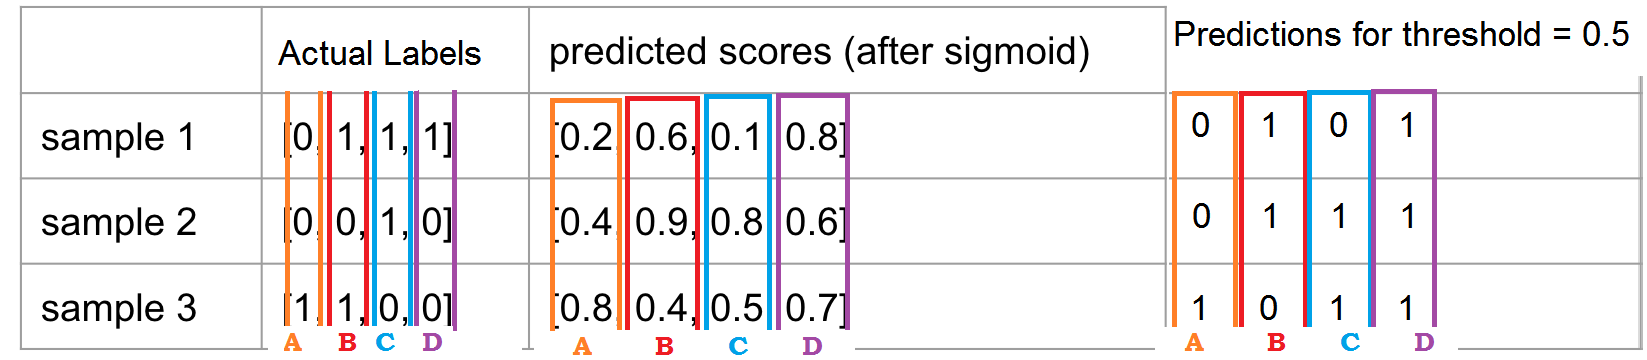
\includegraphics[width=1\textwidth]{figures/evaluate.png}
	\caption{نمونه خروجی مدل و برچسب های داده}
	\label{fig:evaluate}
\end{figure}
در این مثال که لایه انتهایی مدل دارای ۴ نورون می‌باشد. خروجی هر نورون به معنای امتیازی  هست که مدل به آن کلاس مدنظر می‌دهد. خروجی ها ابتدا وارد تابع فعال‌ساز سیگموید\LTRfootnote{sigmoid} می‌شوند تا به احتمالی بین ۰ تا ۱ تبدیل شوند. در آخر با استفاده از حد آستانه‌ای مانند $0.5$ احتمال تبدیل به ۰ و ۱ می‌شوند.
حال می‌توان برای هر کلاس مدنظرتعداد
مثبت صحیح\LTRfootnote{True Positive}،
منفی صحیح\LTRfootnote{False Positive}،
مثبت غلط\LTRfootnote{True Negative}
و منفی غلط\LTRfootnote{False Negative}
را شمارش کرد و با استفاده از روابط \ref{eq:accuracy} تا \ref{eq:ma-f1} مدل را ارزیابی کرد.\cite{BOGATINOVSKI2022117215}

\section{نتایج ارزیابی}

نتایج ارزیابی تشخیص بوی کد بر روی مدل های مختلف در جدول	\ref{tab:performance}
قابل مشاهده است که این مدل ها به اندازه یک دوره بر روی 10000 داده و بیشینه طول ورودی 3000 توکن و با استفاده از \lr{AdamW} به عنوان بهینه گر و از \lr{binary cross-entropy} به عنوان تابغ ضرر آموزش دیده اند.

\begin{table}[H]
	\centering
	\begin{latin}
		\begin{tabular}{lcccc}
			\toprule
			\lr{Model}             & \lr{Precision} & \lr{Recall}  & \lr{Accuracy} & \lr{F1}      \\
			\midrule
			\lr{LLaMA 3.1-8B}      & \lr{36.4555}   & \lr{64.7900} & \lr{75.7842}  & \lr{30.2849} \\
			\lr{gemma 2-9B}        & \lr{35.0419}   & \lr{65.1500} & \lr{73.2184}  & \lr{29.4671} \\
			\lr{LLaMA 3-8B}        & \lr{35.5450}   & \lr{61.9200} & \lr{77.0219}  & \lr{28.5714} \\
			\lr{LLaMA 2-7B}        & \lr{34.0678}   & \lr{64.3900} & \lr{72.1825}  & \lr{28.5714} \\
			\lr{mistral 7B}        & \lr{34.8742}   & \lr{60.4100} & \lr{76.7166}  & \lr{27.8215} \\
			\lr{phi 3.5 mini 3.8B} & \lr{35.0706}   & \lr{60.0100} & \lr{75.8794}  & \lr{28.3837} \\
			\lr{smoLM 2B}          & \lr{35.1047}   & \lr{59.7000} & \lr{73.2540}  & \lr{29.5393} \\
			\lr{GPT2-large}        & \lr{31.8349}   & \lr{61.0300} & \lr{72.6829}  & \lr{25.3835} \\
			\bottomrule
		\end{tabular}
	\end{latin}
	\caption{نتایج ارزیابی مدل های مختلف}
	\label{tab:performance}
\end{table}

\clearpage
